\section*{Kapitel 4 - Diskrete Einflußgrößen}

\begin{multicols*}{3}

\tikzstyle{mybox} = [draw=black, fill=white, very thick,
    rectangle, rounded corners, inner sep=10pt, inner ysep=10pt]
\tikzstyle{fancytitle} =[fill=black, text=white, font=\bfseries]



%------------ Kodierung ---------------
\begin{tikzpicture}
    \node [mybox] (box){%
        \begin{minipage}{0.3\textwidth}
        Sei $C$ eine nominale Variable mit $K$ Ausprägungen.
        \vspace{0.5cm}

        \tc{\textbf{Dummy-Kodierung:}}\\
         Wir definieren $K$ neue Variablen $Z_1, \dots, Z_K$ als
         $$Z_k(C) = \begin{cases} 1, & \text{falls } C = k \\ 0, & \text{sonst} \end{cases}$$
         $Z_1, \dots, Z_K$ sind abhängig, da $Z_K = 1 - \sum_{k=1}^{K-1} Z_k$
        \vspace{0.5cm}

        \tc{\textbf{Effekt-Kodierung:}}
        Wir definieren $K-1$ neue Variablen $Z_1^e, \dots, Z_{K-1}^e$ als
        $$Z_k^e(C) = \begin{cases} 1, & \text{falls } C = k \\ -1, & \text{falls } C = K \\ 0, & \text{sonst} \end{cases}$$
        Note: $Z_k(\bC) = \begin{pmatrix}
            Z_k(C_1) \\ \vdots \\ Z_k(C_n) \end{pmatrix}$ und $Z_k^e(\bC) = \begin{pmatrix}
                Z_k^e(C_1) \\ \vdots \\ Z_k^e(C_n) \end{pmatrix}$
    \end{minipage}
    };
%------------ Kodierung Header ---------------------
\node[fill = black, text=white, font=\bfseries, right=10pt] at (box.north west) 
{Kodierung};
\end{tikzpicture}

%------------ Setup einfache Varianzanalyse ---------------
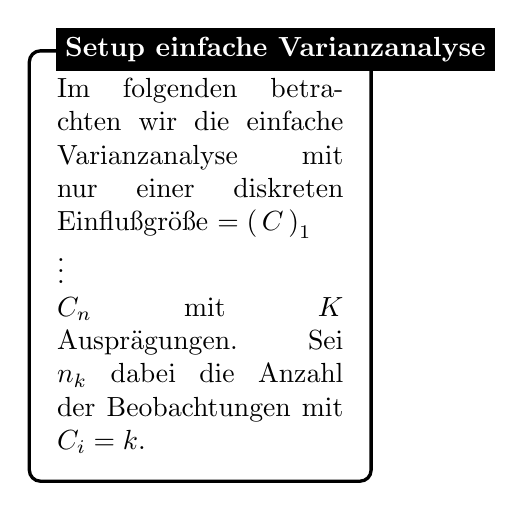
\begin{tikzpicture}
    \node [mybox] (box){%
        \begin{minipage}{0.3\textwidth}
        Im folgenden betrachten wir die einfache Varianzanalyse mit nur einer diskreten Einflußgröße 
        $\bC = \begin{pmatrix} C_1 \\ \vdots \\ C_n \end{pmatrix}$ mit $K$ Ausprägungen.
        Sei $n_k$ dabei die Anzahl der Beobachtungen mit $C_i = k$.
        \end{minipage}
    };
%------------ Setup einfache Varianzanalyse Header ---------------------
\node[fill = black, text=white, font=\bfseries, right=10pt] at (box.north west) 
{Setup einfache Varianzanalyse};
\end{tikzpicture}


%------------ Mittelwertsmodell ---------------
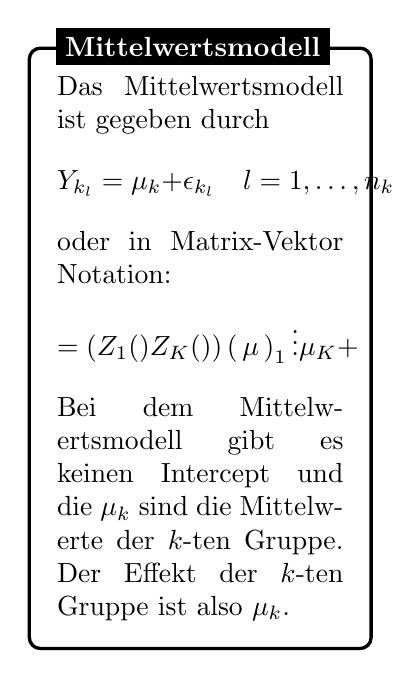
\begin{tikzpicture}
    \node [mybox] (box){%
        \begin{minipage}{0.3\textwidth}
        Das \tc{Mittelwertsmodell} ist gegeben durch
        $$Y_{k_l} = \mu_k + \epsilon_{k_l} \quad l = 1,\dots, n_k \quad k = 1,\dots,K$$
        oder in Matrix-Vektor Notation: 
        $$\bY = (Z_1(\bC) \dotsm Z_K(\bC)) \begin{pmatrix}
            \mu_1 \\ \vdots \\ \mu_K
        \end{pmatrix} + \bepsilon$$
        Bei dem Mittelwertsmodell gibt es keinen Intercept und die $\mu_k$ sind die Mittelwerte der $k$-ten Gruppe.
        Der Effekt der $k$-ten Gruppe ist also $\mu_k$.
        \end{minipage}
    };
%------------ Mittelwertsmodell Header ---------------------
\node[fill = black, text=white, font=\bfseries, right=10pt] at (box.north west) 
{Mittelwertsmodell};
\end{tikzpicture}

%------------ Mittelwertsmodell Beispiel ---------------
\begin{tikzpicture}
    \node [mybox] (box){%
        \begin{minipage}{0.3\textwidth}
        Für $K = 3$ Ausprägungen und $n_k = 2$ für alle $k=1,2,3$ erhalten wir als Mittelwertsmodell:
        $$\bY = \begin{pmatrix} Y_{1_1} \\ Y_{1_2} \\ Y_{2_1} \\ Y_{2_2} \\ Y_{3_1} \\ Y_{3_2}
         \end{pmatrix} = \begin{pmatrix}
            1 & 0 & 0 \\ 1 & 0 & 0 \\ 0 & 1 & 0 \\ 0 & 1 & 0 \\ 0 & 0 & 1 \\ 0 & 0 & 1 \end{pmatrix} \begin{pmatrix}
                \mu_1 \\ \mu_2 \\ \mu_3 \end{pmatrix} + \begin{pmatrix}
                    \eps_{1_1} \\ \eps_{1_2} \\ \eps_{2_1} \\ \eps_{2_2} \\ \eps_{3_1} \\ \eps_{3_2}
        \end{pmatrix}$$
        \end{minipage}
    };
%------------ Mittelwertsmodell Beispiel Header ---------------------
\node[fill = blue, text=white, font=\bfseries, right=10pt] at (box.north west) 
{Mittelwertsmodell Beispiel};
\end{tikzpicture}


%------------ Modell mit Effekt-Kodierung ---------------
\begin{tikzpicture}
    \node [mybox] (box){%
        \begin{minipage}{0.3\textwidth}
        Das \tc{Modell mit Effekt-Kodierung} ist gegeben durch
        $$Y_{k_l} = \mu + \tau_k + \epsilon_{k_l}; \quad \tau_K = -\sum_{k = 1}^{K-1} \tau_k$$ 
        für $\quad l = 1,\dots, n_k \quad k = 1,\dots,K$
        oder in Matrix-Vektor Notation: 
        $$\bY = (\be \hspace{2mm} Z_1^e(\bC) \dotsm Z_{K-1}^e(\bC)) \begin{pmatrix}
            \mu \\ \tau_1 \\ \vdots \\ \tau_{K-1}
        \end{pmatrix} + \bepsilon$$
        Bei dem Modell mit Effekt-Kodierung gibt es einen Intercept $\mu$ und die $\tau_k$ sind die Abweichungen der $k$-ten Gruppe vom Gesamtmittelwert bzw. vom Intercept $\mu$.
        Der Effekt der $k$-ten Gruppe ist also $\mu + \tau_k$.
        \end{minipage}
    };
%------------ Modell mit Effekt-Kodierung Header ---------------------
\node[fill = black, text=white, font=\bfseries, right=10pt] at (box.north west) 
{Modell mit Effekt-Kodierung};
\end{tikzpicture}

%------------ Modell mit Effekt-Kodierung Beispiel ---------------
\begin{tikzpicture}
    \node [mybox] (box){%
        \begin{minipage}{0.3\textwidth}
        Für $K = 3$ Ausprägungen und $n_k = 2$ für alle $k=1,2,3$ erhalten wir als Modell mit Effekt-Kodierung:
        $$\bY = \begin{pmatrix} Y_{1_1} \\ Y_{1_2} \\ Y_{2_1} \\ Y_{2_2} \\ Y_{3_1} \\ Y_{3_2}
         \end{pmatrix} = \begin{pmatrix}
            1 & 1 & 0 \\ 1 & 1 & 0 \\ 1 & 0 & 1 \\ 1 & 0 & 1 \\ 1 & -1 & -1 \\ 1 & -1 & -1 \end{pmatrix} \begin{pmatrix}
                \mu \\ \tau_1 \\ \tau_2  \end{pmatrix}
         + \begin{pmatrix}
            \eps_{1_1} \\ \eps_{1_2} \\ \eps_{2_1} \\ \eps_{2_2} \\ \eps_{3_1} \\ \eps_{3_2} \end{pmatrix}$$
                \end{minipage}
    };
%------------ Modell mit Effekt-Kodierung Beispiel Header ---------------------
\node[fill = blue, text=white, font=\bfseries, right=10pt] at (box.north west) 
{Modell mit Effekt-Kodierung Beispiel};
\end{tikzpicture}

%------------ Modell mit Referenz-Kodierung ---------------
\begin{tikzpicture}
    \node [mybox] (box){%
        \begin{minipage}{0.3\textwidth}
        Das \tc{Modell mit Referenz-Kodierung} ist gegeben durch
        $$Y_{k_l} = \mu_K + \tau_k + \epsilon_{k_l}; \quad \tau_K = 0$$ 
        für $\quad l = 1,\dots, n_k \quad k = 1,\dots,K$
        oder in Matrix-Vektor Notation:
        $$\bY = (\be \hspace{2mm} Z_1(\bC) \dotsm Z_{K-1}(\bC)) \begin{pmatrix}
            \mu_K \\ \tau_1 \\ \vdots \\ \tau_{K-1}
        \end{pmatrix} + \bepsilon$$
        Beim Modell mit Referenz-Kodierung gibt es einen Intercept $\mu_K$ der den Mittelwert der $K$-ten Gruppe angibt und die $\tau_k$ sind die Abweichungen der $k$-ten Gruppe vom Mittelwert der $K$-ten Referenz-Gruppe.
        Der Effekt der $k$-ten Gruppe ist also $\mu_K + \tau_k$ für $k = 1,\dots,K-1$ und $\mu_K$ für $k = K$.
        \end{minipage}
    };
%------------ Modell mit Referenz-Kodierung Header ---------------------
\node[fill = black, text=white, font=\bfseries, right=10pt] at (box.north west) 
{Modell mit Referenz-Kodierung};
\end{tikzpicture}

%------------ Modell mit Referenz-Kodierung Beispiel ---------------
\begin{tikzpicture}
    \node [mybox] (box){%
        \begin{minipage}{0.3\textwidth}
        Für $K = 3$ Ausprägungen und $n_k = 2$ für alle $k=1,2,3$ erhalten wir als Modell mit Referenz-Kodierung:
        $$\bY = \begin{pmatrix} Y_{1_1} \\ Y_{1_2} \\ Y_{2_1} \\ Y_{2_2} \\ Y_{3_1} \\ Y_{3_2}
         \end{pmatrix} = \begin{pmatrix}
            1 & 1 & 0 \\ 1 & 1 & 0 \\ 1 & 0 & 1 \\ 1 & 0 & 1 \\ 1 & 0 & 0 \\ 1 & 0 & 0 \end{pmatrix} \begin{pmatrix}
                \mu_3 \\ \tau_1 \\ \tau_2  \end{pmatrix}
         + \begin{pmatrix}
            \eps_{1_1} \\ \eps_{1_2} \\ \eps_{2_1} \\ \eps_{2_2} \\ \eps_{3_1} \\ \eps_{3_2} \end{pmatrix}$$
                \end{minipage}
    };
%------------ Modell mit Referenz-Kodierung Beispiel Header ---------------------
\node[fill = blue, text=white, font=\bfseries, right=10pt] at (box.north west) 
{Modell mit Referenz-Kodierung Beispiel};
\end{tikzpicture}

%------------ Bemerkungen-Kodierung ---------------
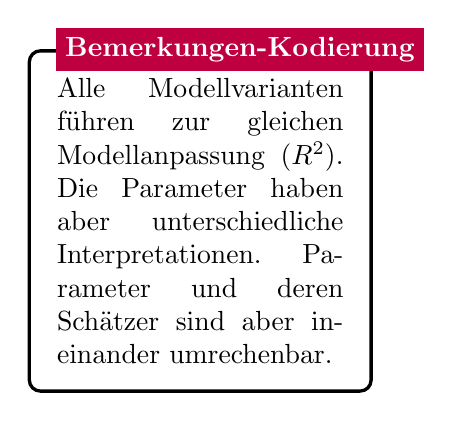
\begin{tikzpicture}
    \node [mybox] (box){%
        \begin{minipage}{0.3\textwidth}
        Alle Modellvarianten führen zur gleichen Modellanpassung ($R^2$).
        Die Parameter haben aber unterschiedliche Interpretationen. Parameter und deren Schätzer sind aber ineinander umrechenbar.
        \end{minipage}
    };
%------------ Bemerkungen-Kodierung Header ---------------------
\node[fill = purple, text=white, font=\bfseries, right=10pt] at (box.north west) 
{Bemerkungen-Kodierung};
\end{tikzpicture}

\newpage

%------------ Setup einfache Varianzanalyse ---------------
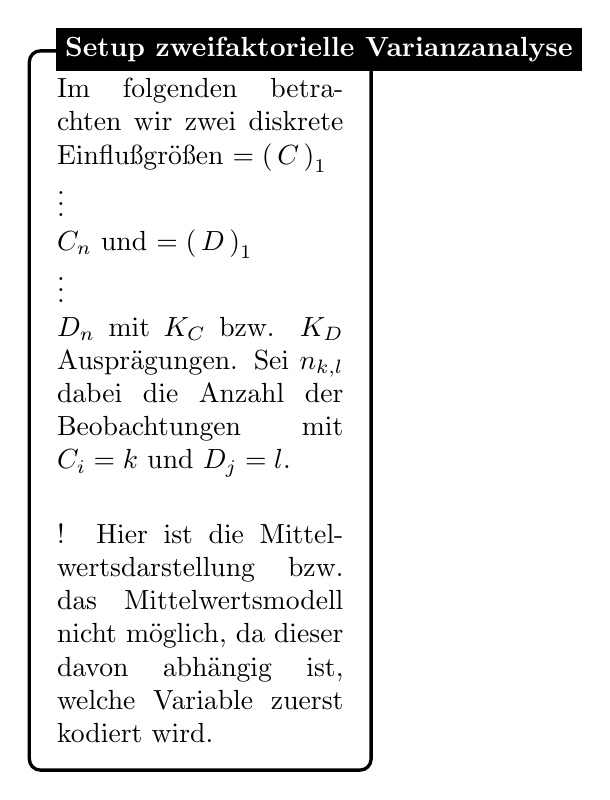
\begin{tikzpicture}
    \node [mybox] (box){%
        \begin{minipage}{0.3\textwidth}
        Im folgenden betrachten wir zwei diskrete Einflußgrößen $\bC = \begin{pmatrix} C_1 \\ \vdots \\ C_n \end{pmatrix}$ und 
        $\bD = \begin{pmatrix} D_1 \\ \vdots \\ D_n \end{pmatrix}$ mit $K_C$ bzw. $K_D$ Ausprägungen.
        Sei $n_{k,l}$ dabei die Anzahl der Beobachtungen mit $C_i = k$ und $D_j = l$.\\
        \vspace{1mm}

        \tc{!} Hier ist die Mittelwertsdarstellung bzw. das Mittelwertsmodell nicht möglich, da dieser davon abhängig ist, welche Variable zuerst kodiert wird.
        \end{minipage}
    };
%------------ Setup einfache Varianzanalyse Header ---------------------
\node[fill = black, text=white, font=\bfseries, right=10pt] at (box.north west) 
{Setup zweifaktorielle Varianzanalyse};
\end{tikzpicture}

%------------ Modell mit Effekt-Kodierung (mehrfaktoriell) ---------------
\begin{tikzpicture}
    \node [mybox] (box){%
        \begin{minipage}{0.3\textwidth}
        Das \tc{Modell mit Effekt-Kodierung} ist gegeben durch
        $$\bY = (\be \hspace{2mm} Z_1^e(\bC) \dotsm Z_{K-1}^e(\bC)) \begin{pmatrix}
            \mu \\ \tau_1 \\ \vdots \\ \tau_{K-1}
        \end{pmatrix} + \bepsilon$$
        Bei dem Modell mit Effekt-Kodierung gibt es einen Intercept $\mu$ und die $\tau_k$ sind die Abweichungen der $k$-ten Gruppe vom Gesamtmittelwert bzw. vom Intercept $\mu$.
        Der Effekt der $k$-ten Gruppe ist also $\mu + \tau_k$.
        \end{minipage}
    };
%------------ Modell mit Effekt-Kodierung (mehrfaktoriell) Header ---------------------
\node[fill = black, text=white, font=\bfseries, right=10pt] at (box.north west) 
{Modell mit Effekt-Kodierung (mehrfaktoriell)};
\end{tikzpicture}

\end{multicols*}